%\begin{figure}[h!]
%    \centering
%    \includegraphics[width=14cm, height= 7.5cm]{.png}
%    \caption{}
%    \label{fig:}
%\end{figure}

%-------------------------------------------------------------------------%
\section{Performance of the classifiers}
%-------------------------------------------------------------------------%
%\subsection{Benchmark 1: \texorpdfstring{$\Tilde{t} = 1.2$}{ } TeV and \texorpdfstring{$\Tilde{\chi}_1^0 = 600$}{ } GeV}
An initial diagnostic tool to understand our classifiers' performance is a simple Receiver Operating Characteristic (ROC) curve. A ROC curve shows the distribution of the predicted values as a function of the FP rate versus the TP rate. This allows us to understand how much error we are willing to accept/reject for a given classifier where we can produce histograms to observe the potential optimum cut-off (see Figures \ref{fig:dist_bm1}-\ref{fig:dist_bm_in}). The ROC curve produced for all four benchmark data is shown in Figure \ref{fig:ROC} with excellent performance across all four. As expected, the benchmark set corresponding to mass parameters within the exclusion curve (Benchmark4: $m_{\Tilde{t}} = 750$ GeV and $m_{\Tilde{\chi}_1^0} = 1$ GeV) performed the worst amongst the four, due to the lighter top squark and a smaller mass difference between the stops and neutralinos. We also note that the classifiers performed better as the mass difference became larger, also an expected behavior as a larger $\Delta m$ creates more energetic stops and tops, consequently, more missing energy. This allowed the classifier to pick up such signatures more easily, and we suspect that the missing energy's magnitude is the most influential variable the classifier has used when performing its splits. \\

\begin{figure}[htbp]
    \centering
    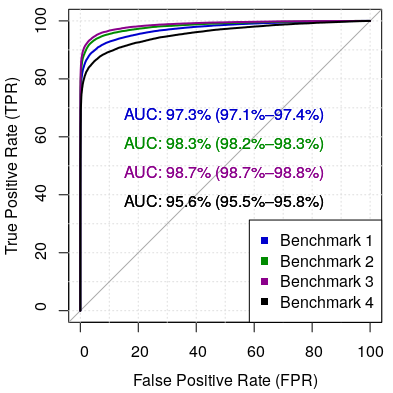
\includegraphics[width=0.45\linewidth]{ROC_curve.png}
    \caption{ROC curve for all 4 benchmark points. The fourth benchmark corresponding to masses within the exclusion curve performed least well, where the remaining three performed slightly better when the mass difference between the stops and neutralinos become larger.}
    \label{fig:ROC}
\end{figure} 

Although the area-under-the-curve (AUC) value is given in Figure \ref{fig:ROC}, it only implies the maximum possible accuracy that the classifier is capable of producing, provided the correct threshold, which does not directly represent the accuracy of our classifiers. The accuracy of our classifiers can be obtained by setting a cut-off to our predictions i.e. a number between 0 and 1. The closer the value is to 1 the lower the accuracy, but deliberately obtaining a high accuracy by setting a smaller value is also counter-intuitive as the SBR for the luminosity-normalized expected events (Equation (\ref{eq:N})) will not be maximized. Through various trials in cut-off values by observing the distribution of the predicted values shown in Figures \ref{fig:dist_bm1}-\ref{fig:dist_bm_in}, it was determined for all four datasets that 0.75 is the optimal value to satisfy both high accuracy and high SBR. A summary of values obtained for each datasets are provided in Tables \ref{tab:Values1}-\ref{tab:Values_in}. 

For the benchmark set with masses $m_{\Tilde{t}} = 1.2$ TeV and $m_{\Tilde{\chi}_1^0} = 600$ GeV, the classifier performed well, producing a result of $91.4 \pm 0.2 \%$ accuracy. As expected, the classifier did not distinguish signal events well as it has for background events as shown in the difference in correctly and incorrectly classifier signal and background events in Table \ref{tab:Values1}. The expected number of signal is significantly less than the expected number of background, producing an AMS value of 0.1 with an SBR of 0.52\%. Both values are extremely small from the overwhelming number of expected background events. Hence, if proper hypothesis tests on either signal-discovery or upper-limits were performed, we can expect neither discovery nor exclusion from these mass parameters. \\

\noindent\begin{minipage}{\textwidth}
\centering
  \begin{minipage}[htbp]{0.6\textwidth}
    \centering
    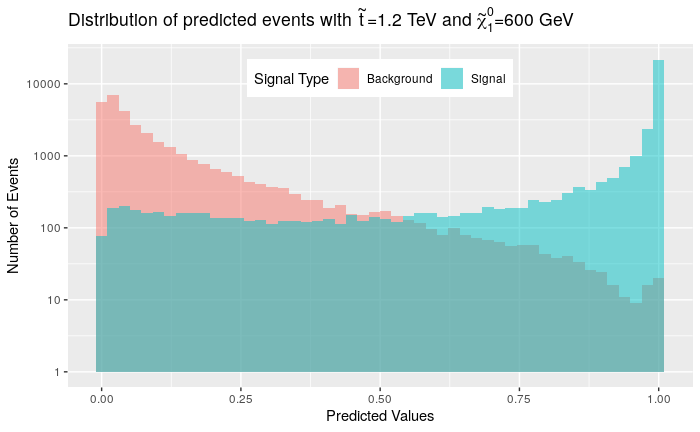
\includegraphics[width=\linewidth]{bm1_distribution.png}
    \captionof{figure}{The distribution of the predicted outcomes for both background (pink) and signal (blue) events. The signal has a sharp drop-off at higher cut-off values unlike the background steadily, almost linearly, decreasing in number toward higher values until a rapid drop-off very close to 1.}
    \label{fig:dist_bm1}
  \end{minipage}
  \hfill\hfill\hfill
  \begin{minipage}[htbp]{0.39\textwidth}
        \centering
        \begin{tabular}{c|c} 
        \toprule
        Metric & Proportion \\
        \midrule
        \rowcolor{gray!6} TP & $42.0 \%$ \\
        TN & $49.4 \%$ \\
        \rowcolor{gray!6} FP & $0.6 \%$\\
        FN & $8.0 \%$ \\
        \rowcolor{gray!6} Accuracy & $91.4 \pm 0.2 \%$ \\
        \midrule
        $b$ & $388$ \\
        \rowcolor{gray!6} $s$ & $2$ \\
        SBR & $0.52\%$\\
        \rowcolor{gray!6} AMS & $0.1$ \\
        \bottomrule
        \end{tabular}
        \captionof{table}{Proportion of correctly and incorrectly classified points with the number of expected events calculated with Equation (\ref{eq:N}). The ratio, SBR, and AMS (Equation (\ref{eq:AMS})) were also calculated.} 
        \label{tab:Values1}
    \end{minipage}
\end{minipage}
\break

%-------------------------------------------------------------------------%
%\subsection{Benchmark 2: \texorpdfstring{$\Tilde{t} = 1.225$}{ } TeV and \texorpdfstring{$\Tilde{\chi}_1^0 = 400$}{ } GeV}

For Benchmarks 2 ($m_{\Tilde{t}} = 1.225$ TeV and $m_{\Tilde{\chi}_1^0} = 400$ GeV) and 3 ($m_{\Tilde{t}} = 1.25$ TeV and $m_{\Tilde{\chi}_1^0} = 100$ GeV) a slight improvement can be seen with the overall accuracy of the classifier, the SBR and AMS values, attributed to the larger mass differences between the stops and neutralinos. As noted in previous sections, the larger mass difference produces much more energetic final states, consequently more missing energy, allowing the classifier to distinguish background and signal events better. This relates to the distribution for $\cancel{\it{E}}_{T}$ shown in Figure \ref{fig:topMET} in Section \ref{sec:production}, where the signal events have a wider distribution with a mean centered further away from the background. This is further supported with the distribution plot in Figure \ref{fig:METs}, where we see the distribution become flatter, wider and further away toward higher $\cancel{\it{E}}_{T}$ values as the mass difference between the stops and neutralinos become larger. \\


\begin{figure}[htbp]
    \centering
    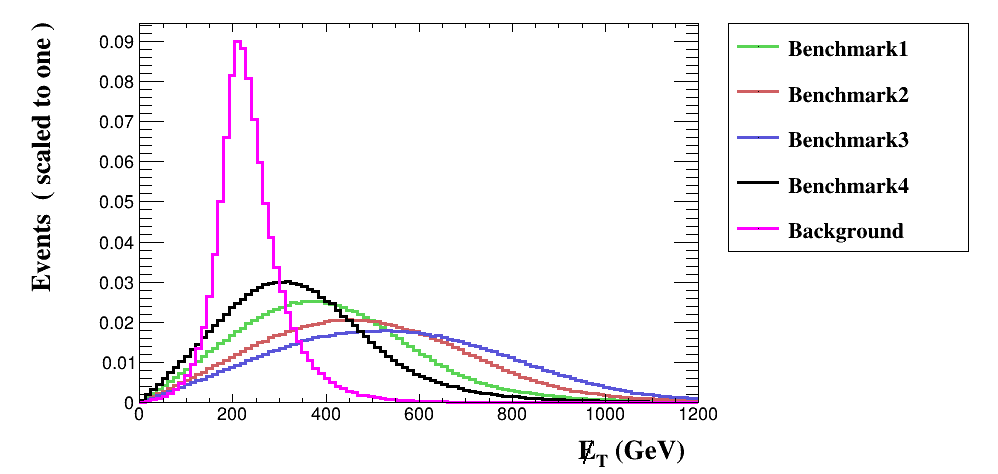
\includegraphics[width=\linewidth]{METs.png}
    \caption{The distribution of $\cancel{\it{E}}_{T}$ for all four signal events and the background events. The distribution shifts toward higher $\cancel{\it{E}}_{T}$ values as $\Delta m = m_{\Tilde{t}} - m_{\Tilde{\chi}_1^0}$ becomes larger. The benchmark corresponding to mass parameters within the exclusion curve (black) has the closest distribution to the background events as the lighter neutralino masses contribute to less $\cancel{\it{E}}_{T}$ within the events.}
    \label{fig:METs}
\end{figure}
\hfill\break
\hfill\break

\noindent\begin{minipage}{\textwidth}
\centering
  \begin{minipage}[htbp]{0.6\textwidth}
    \centering
    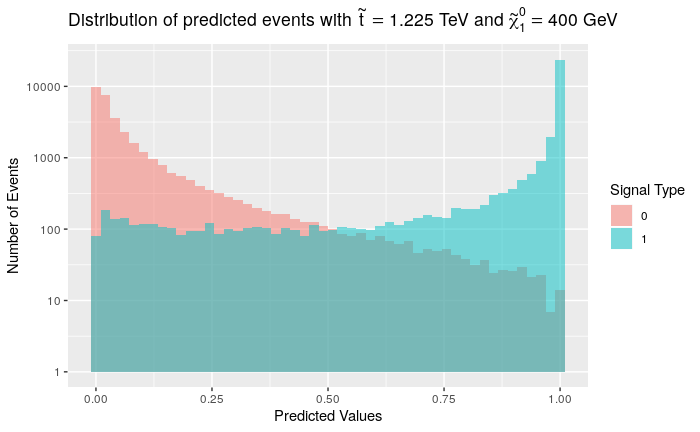
\includegraphics[width=\linewidth]{bm2_distribution.png}
    \captionof{figure}{The distribution of predicted outcomes for Benchmark 2: $m_{\Tilde{t}} = 1.225$ TeV and $m_{\Tilde{\chi}_1^0} = 400$ GeV, similar to Figure \ref{fig:dist_bm1}. }%Distribution of predicted background (pink) and signal (blue) events. The signal has a sharp drop-off at higher cut-off values similarly to the background, wherein the background also decreases rapidly in number toward higher values compared to the signal. There is a slight upward trend for the signal with values closer to zero. } %Note that y-axis is in a $\log_{10}$ scale.}
    \label{fig:dist_bm2}
  \end{minipage}
  \hfill
  \begin{minipage}[htbp]{0.39\textwidth}
        \centering
        \begin{tabular}{c|c} 
        \toprule
        Metric & Proportion \\
        \midrule
        \rowcolor{gray!6} TP & $43.8 \%$ \\
        TN & $49.5 \%$ \\
        \rowcolor{gray!6} FP & $0.5 \%$\\
        FN & $6.2 \%$ \\
        \rowcolor{gray!6} Accuracy & $93.3 \pm 0.2 \%$ \\
        \midrule
        $b$ & $362$ \\
        \rowcolor{gray!6} $s$ & $6$ \\
        SBR & $1.7\%$\\
        \rowcolor{gray!6} AMS & $0.31$ \\
        \bottomrule
        \end{tabular}
        \captionof{table}{The proportion of correctly and incorrectly classified points, the expected number of background and signal events with the calculated SBR and AMS, as per Table \ref{tab:Values2}.} 
        \label{tab:Values2}
    \end{minipage}
\end{minipage}
\hfill\break
\hfill\break
\hfill\break
%-------------------------------------------------------------------------%
%\subsection{Benchmark 3: \texorpdfstring{$\Tilde{t} = 1.25$}{ } TeV and \texorpdfstring{$\Tilde{\chi}_1^0 = 100$}{ } GeV}

\noindent\begin{minipage}{\textwidth}
\centering
  \begin{minipage}[htbp]{0.6\textwidth}
    \centering
    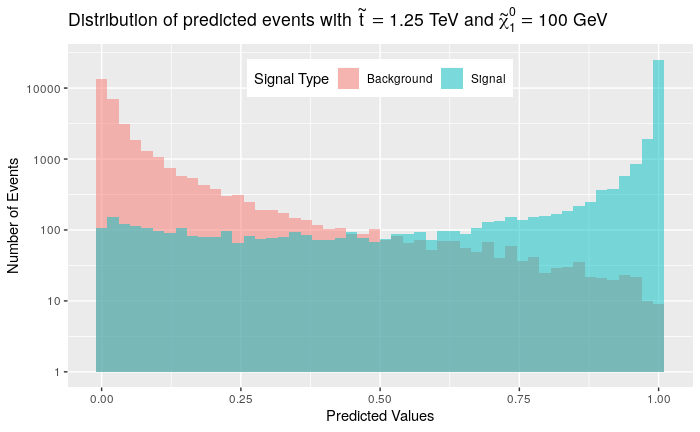
\includegraphics[width=\linewidth]{bm3_distribution.png}
    \captionof{figure}{The distribution of predicted outcomes for Benchmark 3: $m_{\Tilde{t}} = 1.25$ TeV and $m_{\Tilde{\chi}_1^0} = 100$ GeV, similar to Figure \ref{fig:dist_bm1}. }%Distribution of predicted background (pink) and signal (blue) events. The signal has a sharp drop-off at higher cut-off values similarly to the background, wherein the background also decreases rapidly in number toward higher values compared to the signal. There is a slight upward trend for the signal with values closer to zero.}
    \label{fig:dist_bm3}
  \end{minipage}
  \hfill
  \begin{minipage}[htbp]{0.39\textwidth}
        \centering
        \begin{tabular}{c|c} 
        \toprule
        Metric & Proportion \\
        \midrule
        \rowcolor{gray!6} TP & $44.9 \%$ \\
        TN & $49.5 \%$ \\
        \rowcolor{gray!6} FP & $0.5 \%$\\
        FN & $5.1 \%$ \\
        \rowcolor{gray!6} Accuracy & $94.4 \pm 0.2 \%$ \\
        \midrule
        $b$ & $323$ \\
        \rowcolor{gray!6} $s$ & $11$ \\
        SBR & $3.4\%$\\
        \rowcolor{gray!6} AMS & $0.6$ \\
        \bottomrule
        \end{tabular}
        \captionof{table}{The proportion of correctly and incorrectly classified points, the expected number of background and signal events with the calculated SBR and AMS, as per Table \ref{tab:Values2}.} 
        \label{tab:Values3}
    \end{minipage}
\end{minipage}
\hfill\break
\hfill\break
%-------------------------------------------------------------------------%
%\subsection{Benchmark 4: \texorpdfstring{$\Tilde{t} = 750$}{ } GeV and \texorpdfstring{$\Tilde{\chi}_1^0 = 1$}{ } GeV}
\indent For the mass parameters within the exclusion curve, $m_{\Tilde{t}} = 750$ GeV and $m_{\Tilde{\chi}_1^0} = 1$ GeV, the accuracy drops below 90\% with the given cut-off as shown in Table \ref{tab:Values_in}. This shows that 20\% of the signal events were misclassified (10\% of total data) which is concerning as it produces a larger SBR value at 15.7\%. The AMS value of 2.8 obtained by this dataset is higher than the value found by reference \cite{roxlo2018opening}, given as 1.72. This seems too high for a point already excluded by CMS experiments, thus as a check, we calculated the relevant values with the same luminosity value as in \cite{roxlo2018opening} where $\text{I.L.}=35.9\text{ fb}^{-1}$. We obtained an AMS value of 1.37 with an associated SBR value of 15.6\%, a much closer AMS value to that in \cite{roxlo2018opening}. This assures that this mass parameter is indeed excluded which also adds further support to the AMS being a viable metric for searches in collider physics. It is worth noting that different luminosity value affects the calculation of the AMS greatly, but does not affect the statistical nature of our data and analysis. \\

%Despite the large AMS value, we remain with a relatively low SBR value at 15.7\%, which is a reassuring result as it supports the exclusion limit shown in Figure \ref{fig:limits} that indeed this point is unlikely to be the mass parameters for both the stop and the neutralino interesting characteristic to observe when we visualise the data in the next section. 
\noindent\begin{minipage}{\textwidth}
  \centering
  \begin{minipage}[htbp]{0.6\textwidth}
    \centering
    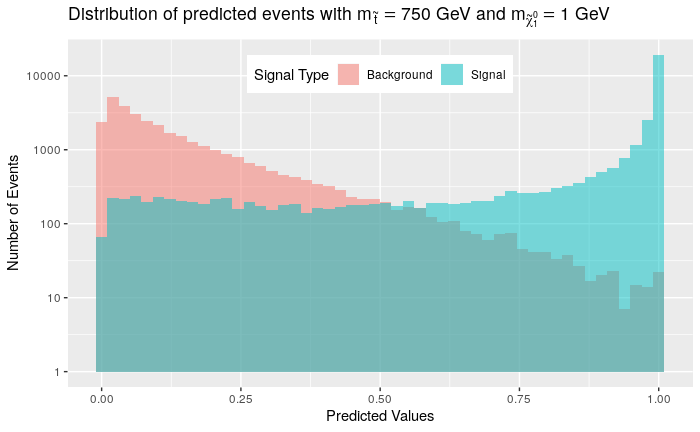
\includegraphics[width=\linewidth]{bm_In_distribution.png}
    \captionof{figure}{The distribution of predicted outcomes for Benchmark 3: $m_{\Tilde{t}} = 750$ GeV and $m_{\Tilde{\chi}_1^0} = 1$ GeV, similar to Figure \ref{fig:dist_bm1}.}
    \label{fig:dist_bm_in}
  \end{minipage}
  \hfill
  \begin{minipage}[htbp]{0.39\textwidth}
        \centering
        \begin{tabular}{c|c} 
        \toprule
        Metric & Proportion \\
        \midrule
        \rowcolor{gray!6} TP & $39.4 \%$ \\
        TN & $49.6 \%$ \\
        \rowcolor{gray!6} FP & $0.4 \%$\\
        FN & $10.6 \%$ \\
        \rowcolor{gray!6} Accuracy & $89.0 \pm 0.2 \%$ \\
        \midrule
        $b$ & $343$ \\
        \rowcolor{gray!6} $s$ & $54$ \\
        SBR & $15.7\%$\\
        \rowcolor{gray!6} AMS & $2.8$ \\
        \bottomrule
        \end{tabular}
        \captionof{table}{The proportion of correctly and incorrectly classified points, the expected number of background and signal events with the calculated SBR and AMS, as per Table \ref{tab:Values2}.} 
        \label{tab:Values_in}
    \end{minipage}
\end{minipage}

\begin{table}[htbp]
    \centering
    \begin{tabular}{c||c|c}
        \toprule
        Metric & I.L. = $137\text{ fb}^{-1}$ & I.L. = $35.9\text{ fb}^{-1}$ \\
        \midrule
        \rowcolor{gray!6} $b$ & $343$ & $90$ \\
        $s$ & $54$ & $14$\\
        \rowcolor{gray!6} SBR & $15.7\%$ & $15.6\%$\\
        AMS & $2.8$ & $1.37$ \\
        \bottomrule
    \end{tabular}
    \caption{A table comparing values obtained with two different values for the integrated luminosity (I.L.), $137\text{fb}^{-1}$ and $35.9\text{fb}^{-1}$, within the mass parameter $\Tilde{t} = 750$ GeV and $\Tilde{\chi}_1^0 = 1$ GeV. Although the AMS values differ the SBR is almost identical, showing that the increase in luminosity helps in adding sensitivity to the searches.}
    \label{tab:valsComp}
\end{table}

%XGBoost has an additional useful feature that calculates the \textit{feature importance} according to the \textit{Gain}, \textit{Cover} and \textit{Frequency} of each variable fed into building the classifiers \cite{xgboost}. We have used the metric `Gain' as it corresponds to the contribution of each variable based on the total gain they had when performing splits. We plot the variables accordingly, shown in Figure \ref{fig:imps} below. \\

With the numerical results obtained from the classifiers, we now turn feature importance\footnote{See section \ref{sec:importance}.} From the bar-plots shown in Figure \ref{fig:imps}, the highest contribution consistently comes from the variable $\cancel{\it{E}}_{T}$ thus making it the most important. This is expected as we know that the neutralinos and the SM neutrinos produced from the highly energetic top quarks in our signal events contribute to more $\cancel{\it{E}}_{T}$. The next highest contributors were the $\phi$ components of $\cancel{\it{E}}_{T}$ and the lepton as well as its $p_T$, followed by the hadronic energy $H_T$. These five variables were consistently the top-five contributors, and observing the groups (noted as clusters, groupings of variables with similar importance), we can infer that in particular, the $\phi$ components of $\cancel{\it{E}}_{T}$ and the lepton have some sort of correlation with an occasional contribution from the lepton's $p_T$. We also observe that the $p_T$ of the $b$-jet and the remaining jet with the highest $p_T$ (referred to as jet-1 henceforth) occasionally have a slight contribution to the algorithm, with the remaining variables considered almost irrelevant consistently.

\begin{figure}[htbp]
\centering
  \begin{minipage}[htbp]{0.49\textwidth}
    \centering
    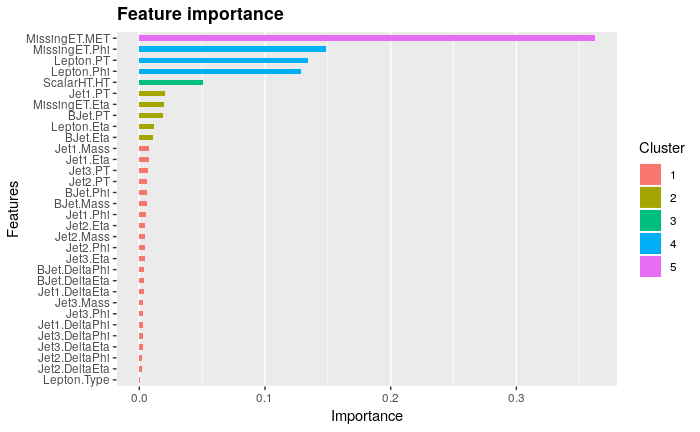
\includegraphics[width=\linewidth, keepaspectratio=true]{imp1.png}
  \end{minipage}
  \hfill
  \begin{minipage}[htbp]{0.49\textwidth}
    \centering
    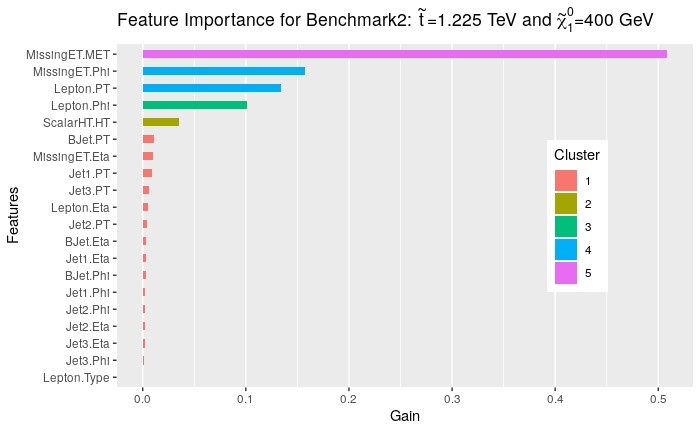
\includegraphics[width=\linewidth, keepaspectratio=true]{imp2.png}
  \end{minipage}
  \hfill
  \begin{minipage}[htbp]{0.49\textwidth}
    \centering
    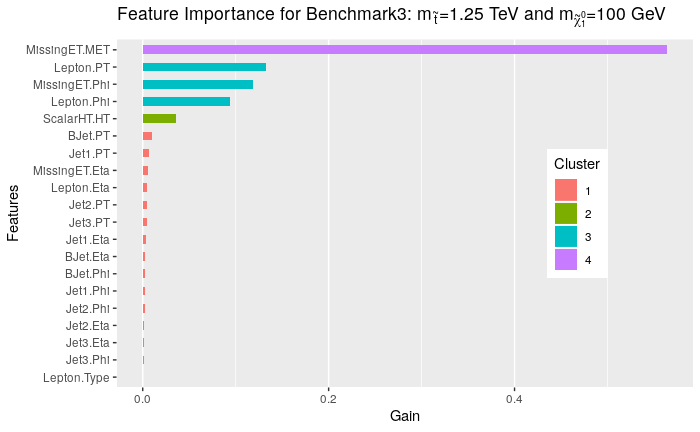
\includegraphics[width=\linewidth, keepaspectratio=true]{imp3.png}
  \end{minipage}
  \hfill
  \begin{minipage}[htbp]{0.49\textwidth}
    \centering
    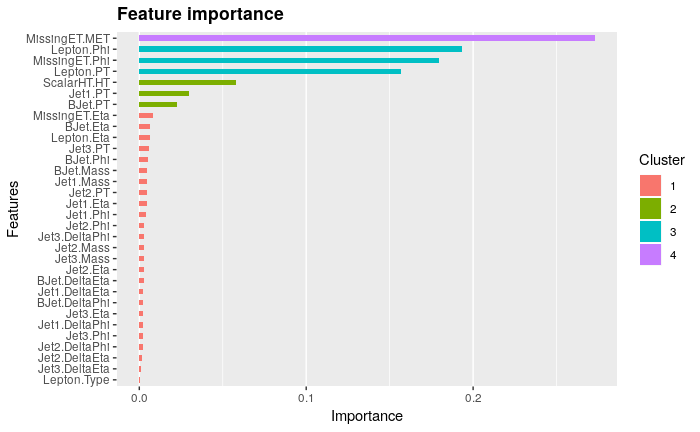
\includegraphics[width=\linewidth, keepaspectratio=true]{imp_in.png}
  \end{minipage}
  \caption{The feature importance for all four benchmark points ordered from top-left to bottom-right. All four classifiers considers $\cancel{\it{E}}_{T}$ the most important feature, followed by the $\phi$ component of $\cancel{\it{E}}_{T}$ and the lepton as well as the lepton's $p_T$, not necessarily in this order. Furthermore the fifth most important variable is $H_T$ opposed to a particular jet's $p_T$. The clustering helps us to undestand the which variables were grouped together when considering a split.}
  \label{fig:imps}
\end{figure}

%-------------------------------------------------------------------------%
\section{Data Visualisation using \textit{tourr}}
In this section, we present how data visualisation could be useful in helping to better understand new physics beyond the SM. Scatter-plots are a good tool to analyse relationships between two variables, but it becomes more difficult to infer results for multiple variables simultaneously. By considering scatter-plots as a two-dimensional projection of a pair of variables, scatter-plots with multiple variables are a projection of the hypercube containing multiple variables. A single projection seen in methods such as principle component analysis is most likely not helpful in the first try, hence the \textit{tourr} package from R \cite{tourr} is an ideal program, in which a sequence of related projections are combined to form a \textit{guided tour}. \\

The guided tour requires an index to pursue `interesting' projections, in which we chose to use the \textit{alpha-hull}\footnote{The alpha-hull index was developed by a student who worked with my supervisors in an undergraduate research project.} index. The alpha-hull is a form of the convex hull that creates convex envelopes around a group of points in the data, in which the alpha value reduces the area connecting points as much as possible. The index uses this property and observes how many points from a different group falls within the alpha-shape. The goal of the guided tour is to apply the index and find a projection that separates distinguished groups in the data. In our case, we hoped to observe distinct groupings of the signal and background events that can help us identify structures related to physical information about the process. Each projection generated gives a basis as a matrix and the algorithm searches through potentially optimal projections in iterations. The complete tour path is then a list of $v\times2$ matrices for the total number of basis created, where $v$ is the number of input variables. \\

From the preceding section, we observed in Figure \ref{fig:imps} that the five most important variables were the energy and $\phi$ components of both the $\cancel{\it{E}}_{T}$ and the charged leptons, and the hadronic energy $H_T$. As the final state of interest included four jets, one of which originated from a $b$-quark, I included the $p_T$ of the $b$-jet and jet-1 as variables worth exploring in our tours. For the tours created in Figures \ref{fig:bmIn_tour}\textemdash\ref{fig:bm3F_tour}, these variables are denoted as follows:

\begin{itemize}
    \item Missing Transver Energy = MissingET.MET (MET.M)
    \item Charged lepton $p_T$ = Lepton.PT (L.PT)
    \item Azimuthal component of MET = MissingET.Phi (MET.P)
    \item Azimuthal component of charged leptons = Lepton.Phi (Lp.P)
    \item Hadronic Energy $H_T$ = ScalarHT.HT (SHT)
    \item $b$-jet $p_T$ = BJet.PT (BJ.)
    \item $p_T$ of jet-1 = Jet1.PT (J1.)
\end{itemize}

Two separate tours were created for two of the benchmark sets chosen to be Benchmarks 3 ($m_{\Tilde{t}} = 1.25$ TeV and $m_{\Tilde{\chi}_1^0} = 100$ GeV) and 4 ($m_{\Tilde{t}} = 750$ GeV and $m_{\Tilde{\chi}_1^0} = 1$ GeV). The first tour was created from extracting 1/10 of the data with the predicted outcomes (both correctly and incorrectly classified background and signal), highlighting each prediction with different colors. The other tour was created only the misclassified points extracted from the partitioned set to observe where the classifiers struggled and what properties it may have. For the former, we color the correctly classified signal and background as blue and black, respectively, and the misclassified signal and background as red and green, respectively. The latter tour has the misclassified signal and background as red and blue respectively. \\

We notice from Figures \ref{fig:bmIn_tour} and \ref{fig:bm3_tour}, the most interesting projections seen were in the form of flattened `M' shapes where the background events were distinctly grouped in three along with the azimuthal components of MET and charged leptons. As each entry in our data is scaled to values in $(0,1)$, negative valued entries are closest to the origin meaning that background events tend to have a large $\phi$ in both the negative and positive direction. Since the coverage of $\phi$ is $-\pi \le \phi \le \pi$ within the detector, it suggest that background events prefer to be close to an orthogonal direction to the $x$-axis, almost as though in a small `cone' forming between the lepton and missing energy, to the beam axis with relatively low $\cancel{\it{E}}_{T}$. In contrast, the signal events have a much larger spread in both $\cancel{\it{E}}_{T}$ and both azimuthal components. This implies that such events are detected almost anywhere within the detector except for the $x$-direction orthogonal to the beam, suggesting a much larger `cone' forming between the lepton and missing energy. \\

\begin{figure}[htbp]
\centering
  \begin{minipage}[htbp]{0.4\textwidth}
    \centering
    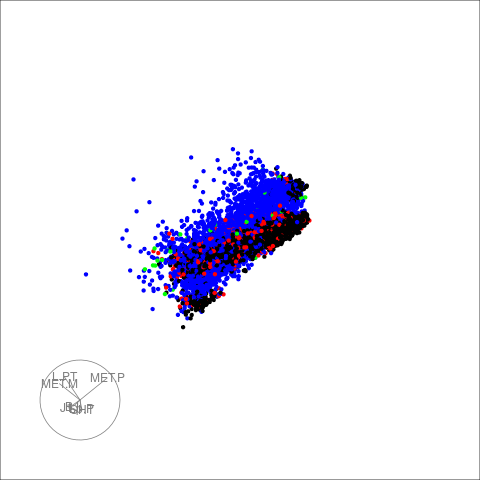
\includegraphics[width=\linewidth, keepaspectratio=true]{bm_I_proper-001.png}
  \end{minipage}
  \begin{minipage}[htbp]{0.4\textwidth}
    \centering
    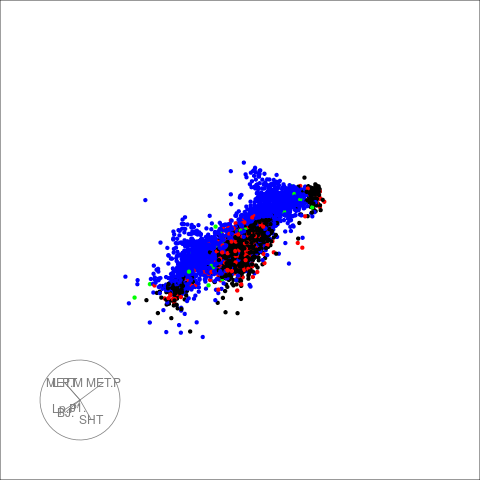
\includegraphics[width=\linewidth, keepaspectratio=true]{bm_I_proper-013.png}
  \end{minipage}
  \begin{minipage}[htbp]{0.4\textwidth}
    \centering
    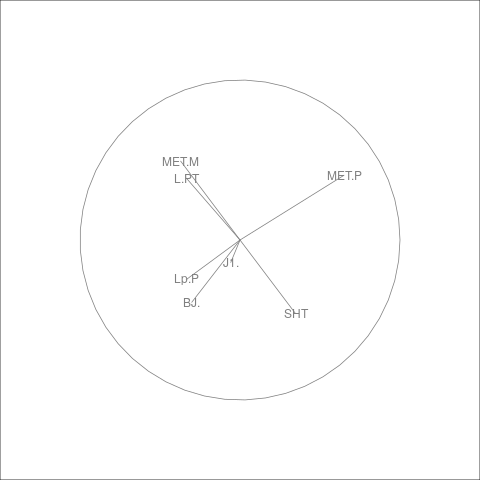
\includegraphics[width=\linewidth, keepaspectratio=true]{bm_I_proper_axis.png}
  \end{minipage}
  \begin{minipage}[htbp]{0.4\textwidth}
    \centering
    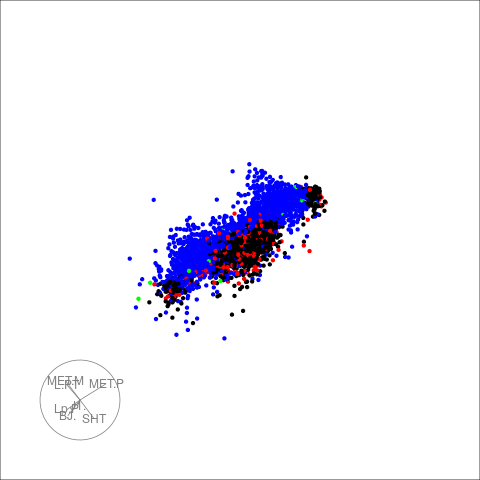
\includegraphics[width=\linewidth, keepaspectratio=true]{bm_I_proper-025.png}
  \end{minipage}
  \caption{Guided tour of predicted points in  Benchmark 4: $m_{\Tilde{t}} = 750$ GeV and $m_{\Tilde{\chi}_1^0} = 1$ GeV. The signal events are colored in blue and red for correctly and incorrectly classified points, respectively. The remaining black and green points correspond to the correctly and incorrectly classified background events, respectively. We observe a flat `M' shape with the true background events grouped into three different regions along the azimuthal variables.}
  \label{fig:bmIn_tour}
\end{figure}

\begin{figure}[htbp]
\centering
  \begin{minipage}[htbp]{0.4\textwidth}
    \centering
    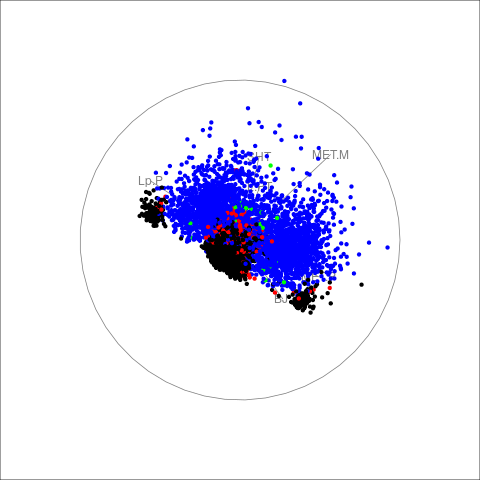
\includegraphics[width=\linewidth, keepaspectratio=true]{bm3_proper-001.png}
  \end{minipage}
  \begin{minipage}[htbp]{0.4\textwidth}
    \centering
    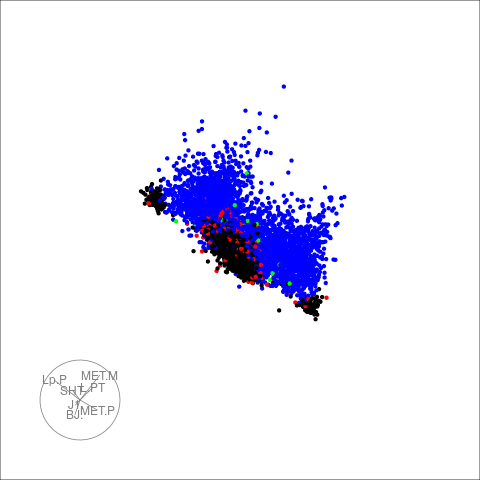
\includegraphics[width=\linewidth, keepaspectratio=true]{bm3_proper-012.png}
  \end{minipage}
  \begin{minipage}[htbp]{0.4\textwidth}
    \centering
    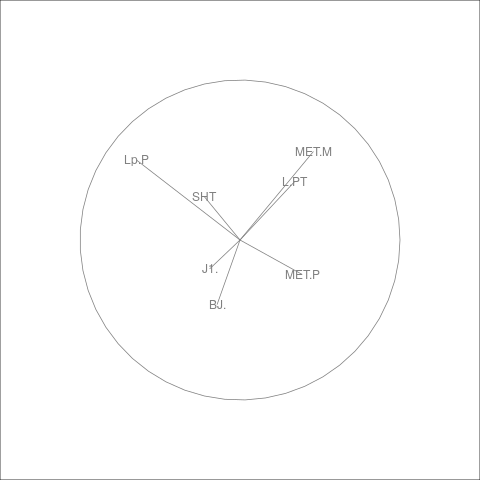
\includegraphics[width=\linewidth, keepaspectratio=true]{bm3_proper_axis.png}
  \end{minipage}
  \begin{minipage}[htbp]{0.4\textwidth}
    \centering
    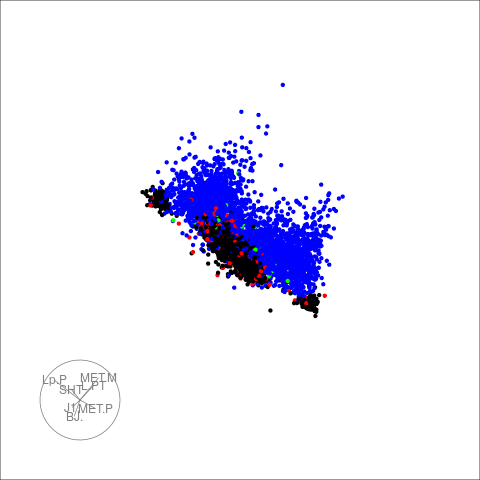
\includegraphics[width=\linewidth, keepaspectratio=true]{bm3_proper-020.png}
  \end{minipage}
  \caption{Guided tour of predicted points in Benchmark 3: $m_{\Tilde{t}} = 1.25$ TeV and $m_{\Tilde{\chi}_1^0} = 100$ GeV. The signal events are colored in blue and red for correctly and incorrectly classified points, respectively. The remaining black and green points correspond to the correctly and incorrectly classified background events, respectively. We observe a flat `M' shape with the true background events grouped into three different regions along the azimuthal variables, identical to that of Figure \ref{fig:bmIn_tour}.}
  \label{fig:bm3_tour}
\end{figure}

\newpage

To further analyse the relationship between the $\phi$ component of the $\cancel{\it{E}}_{T}$ and the charged lepton, we construct a new variable $\Delta \phi(\cancel{\it{E}}_{T},l)$ whose distribution for the signal and background events are shown in Figure \ref{fig:dphi}. The background events indeed favor the narrow separation, whereas the signal events are distributed across the whole range $-\pi \leq \phi \leq \pi$. The broader distribution stems from the neutralino production that is measured at an arbitrary angle relative to the leptons and neutrino, hence a narrower separation will be easily misclassified by ML algorithms. \\

\begin{figure}[htbp]
\centering
  %\begin{minipage}[htbp]{0.4\textwidth}
  %  \centering
  %  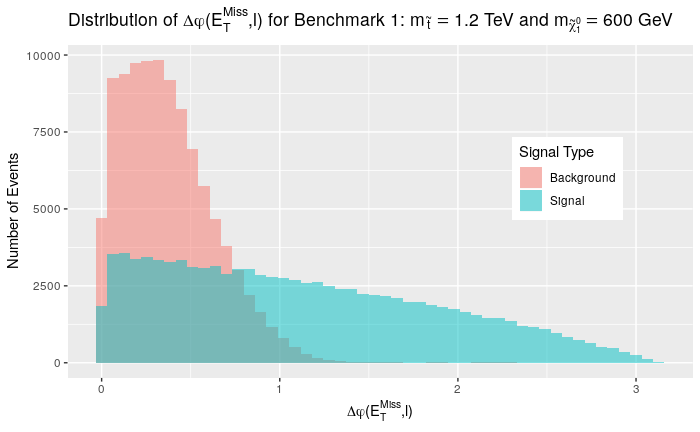
\includegraphics[width=\linewidth, keepaspectratio=true]{dphi_bm1.png}
  %\end{minipage}
  %\begin{minipage}[htbp]{0.4\textwidth}
    %\centering
   % 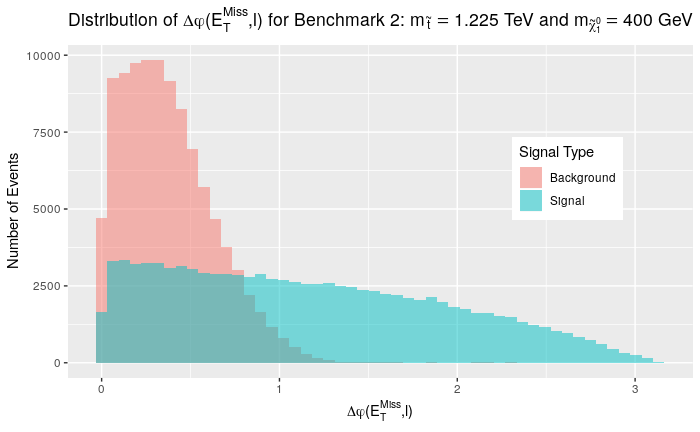
\includegraphics[width=\linewidth, keepaspectratio=true]{dphi_bm2.png}
  %\end{minipage}
  \begin{minipage}[htbp]{\textwidth}
    \centering
    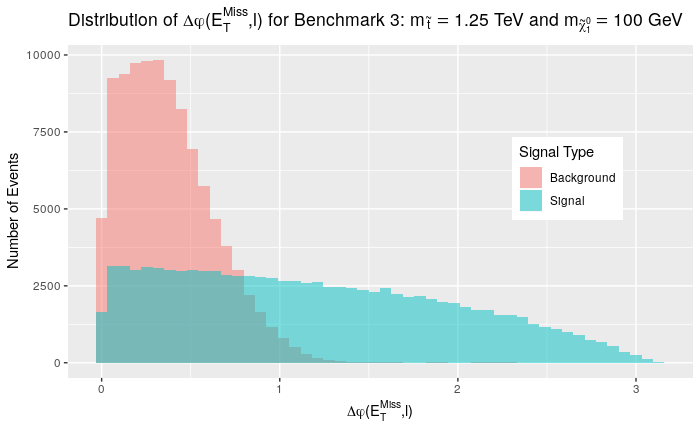
\includegraphics[width=0.65\linewidth, keepaspectratio=true]{dphi_bm3.png}
  \end{minipage}
  \begin{minipage}[htbp]{\textwidth}
    \centering
    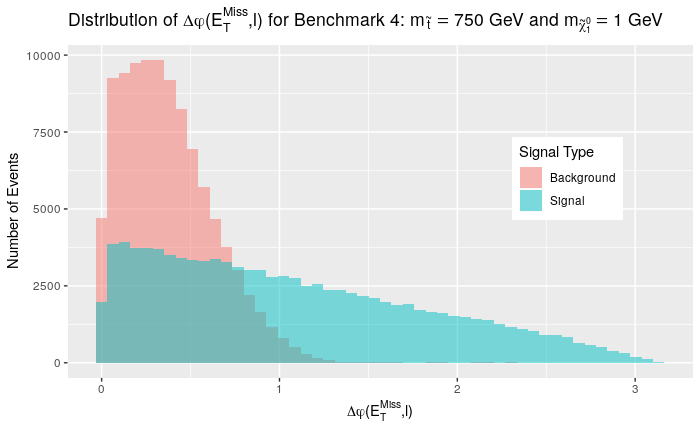
\includegraphics[width=0.65\linewidth, keepaspectratio=true]{dphi_bm_In.png}
  \end{minipage}
  \caption{The distribution of the difference in the $\phi$ component of $\cancel{\it{E}}_{T}$ and the charged lepton, $\Delta \phi(\cancel{\it{E}}_{T},l)$, for both signal (blue) and background (pink) events. Above is the distribution in $m_{\Tilde{t}} = 1.25$ GeV and $m_{\Tilde{\chi}_1^0} = 100$ GeV, and below is the distribution in $m_{\Tilde{t}} = 750$ GeV and $m_{\Tilde{\chi}_1^0} = 1$ GeV. The signal events show a broader distribution than the background events that have a smaller separation between the neutrino and the charged lepton. The broader variation in signal events can be attributed to the neutralino that can be `measured' at a completely arbitrary angle.}
  \label{fig:dphi}
\end{figure}

\newpage
By manually tracing some of the misclassified points from tours created as those shown in Figures \ref{fig:bmInF_tour} and \ref{fig:bm3F_tour}, we can inspect the signal- and background-like signatures that caused the classifiers to perform poorly. A summary of some example values are shown in Tables \ref{tab:ex_bmI} and \ref{tab:ex_bm3}. We observed that the signal-like events were highly energetic in its final states as expected, with the missing energy ranging from 300 GeV to just under 1 TeV. However, we also notice that the $\phi$ range is similar in both signatures, as discussed in the preceding paragraph, with a very narrow separation $\Delta \phi(\cancel{\it{E}}_{T},l)$. We also observed that the energy sum of jets $H_T$ has a large variance, ranging from a few hundred GeV to the order of a few TeV. As a consequence, the jets can be highly energetic with the $b$-jet and jet1 having $p_T$ values interchanging in which has the higher energy between the two. If the $b$-jet is the more energetic jet, we see a less energetic charged lepton detected for the specific event, whereas a highly energetic $b$-jet corresponds to a less energetic charged lepton detected. This is no surprise as we see energy conserved for the SM top quark decay which is part of our final state, hence, combined with the spread across varying energies for both misclassified events, it is understandable that the classifier could not distinguish these events well. \\


\begin{table}[htbp]
    \centering
    \begin{tabular}{p{2.2cm}||c|c|c|c|c|c|c|c|c}
        \toprule
    %----------------------------------%
        \textbf{Signature} & $\cancel{\it{E}}_{T}$ & $\phi(\cancel{\it{E}}_{T})$ & $l$ & $p_T(l)$ & $\phi(l)$ & $H_T$ & $p_T(b)$ & $p_T(j1)$ & $\Delta \phi(\cancel{\it{E}}_{T},l)$ \\
        \midrule
        \multirow{3.75}{*}{Signal-like} & \cellcolor{gray!6}740.57 & \cellcolor{gray!6}0.04 & \cellcolor{gray!6}$\mu$ & \cellcolor{gray!6}380.57 & \cellcolor{gray!6}-0.16 & \cellcolor{gray!6}2719.36 & \cellcolor{gray!6}925.04 & \cellcolor{gray!6}1281.41 & \cellcolor{gray!6}0.12 \\
        %-------------------------------------------------------------%
        & 843.66 & 2.89 & $e$ & 63.78 & 2.82 & 1127.72 & 1024.26 & 39.68 & 0.07 \\
        %-------------------------------------------------------------%
        &\cellcolor{gray!6}362.58 & \cellcolor{gray!6}-0.25 & \cellcolor{gray!6}$\mu$ & \cellcolor{gray!6}37.85 & \cellcolor{gray!6}-1.49 & \cellcolor{gray!6}615.33 & \cellcolor{gray!6}69.28 & \cellcolor{gray!6}239.62 & \cellcolor{gray!6}1.24 \\
        %-------------------------------------------------------------%
        & 356.79 & 1.25 & $\mu$ & 417.83 & 1.21 & 1333.38 & 847.59 & 67.96 & 0.04 \\
        %-------------------------------------------------------------%
        \midrule
        \multirow{3.75}{*}{\parbox{2.2cm}{Background-like}}&\cellcolor{gray!6}462.91 & \cellcolor{gray!6}2.69 & \cellcolor{gray!6}$\mu$ & \cellcolor{gray!6}518.60 & \cellcolor{gray!6}2.82 & \cellcolor{gray!6}1847.63 & \cellcolor{gray!6}75.55 & \cellcolor{gray!6}1114.09 & \cellcolor{gray!6}0.13 \\
        %-------------------------------------------------------------%
        & 356.21 & -1.58 & $e$ & 109.99 & -1.16 & 739.36 & 41.39 & 389.98 & 0.38 \\
        %-------------------------------------------------------------%
        &\cellcolor{gray!6}271.57 & \cellcolor{gray!6}-2.82 & \cellcolor{gray!6}$\mu$ & \cellcolor{gray!6}40.24 & \cellcolor{gray!6}2.63 & \cellcolor{gray!6}636.15 & \cellcolor{gray!6}94.691 & \cellcolor{gray!6}118.94 & \cellcolor{gray!6}0.19 \\
        %-------------------------------------------------------------%
        & 520.38 & 1.58 & $e$ & 20.05 & 0.89 & 670.81 & 220.37 & 339.69 & 0.69 \\
        \bottomrule
    \end{tabular}
    \caption{Some example values, in GeV (except for $\phi$), for signal- and background-like signatures in the misclassified points for Benchmark4: $m_{\Tilde{t}} = 750$ GeV and $m_{\Tilde{\chi}_1^0} = 1$ GeV.}
    \label{tab:ex_bmI}
\end{table}

\begin{table}[htbp]
    \centering
    \begin{tabular}{p{2.2cm}||c|c|c|c|c|c|c|c|c}
        \toprule
        %&\multicolumn{1}{c|}{\bfseries Benchmark1}  &
        %\multicolumn{1}{c|}{\bfseries Benchmark2}  &
        %\multicolumn{1}{c|}{\bfseries Benchmark3} &
        %\multicolumn{1}{c}{\bfseries Benchmark4} \\
        %\midrule
        %\multirow{2}{1.4cm}{squarks}$\cancel{\it{E}}_{T}$
    %----------------------------------%
        \textbf{Signature} & $\cancel{\it{E}}_{T}$ & $\phi(\cancel{\it{E}}_{T})$ & $l$ & $p_T(l)$ & $\phi(l)$ & $H_T$ & $p_T(b)$ & $p_T(j1)$ & $\Delta \phi(\cancel{\it{E}}_{T},l)$ \\
        \midrule
        \multirow{3.75}{*}{Signal-like} & \cellcolor{gray!6}754.29 & \cellcolor{gray!6}2.87 & \cellcolor{gray!6}$\mu$ & \cellcolor{gray!6}131.05 & \cellcolor{gray!6}2.69 & \cellcolor{gray!6}1816.95 & \cellcolor{gray!6}1172.39 & \cellcolor{gray!6}266.44 & \cellcolor{gray!6}0.18 \\
        %-------------------------------------------------------------%
        & 998.99 & 2.42 & $\mu$ & 263.60 & 2.30 & 2214.59 & 123.67 & 608.16 & 0.12 \\
        %-------------------------------------------------------------%
        &\cellcolor{gray!6}317.86 & \cellcolor{gray!6}-0.03 & \cellcolor{gray!6}$\mu$ & \cellcolor{gray!6}514.17 & \cellcolor{gray!6}-0.23 & \cellcolor{gray!6}1324.56 & \cellcolor{gray!6}733.18 & \cellcolor{gray!6}77.22 & \cellcolor{gray!6}0.20	\\
        %-------------------------------------------------------------%
        & 401.37 & 0.92 & $\mu$ & 21.13 & -1.67 & 646.53 & 72.58 & 416.22 & 0.75 \\
        %-------------------------------------------------------------%
        \midrule
        \multirow{3.75}{*}{\parbox{2.2cm}{Background-like}}&\cellcolor{gray!6}251.72  & \cellcolor{gray!6}2.25 & \cellcolor{gray!6}$\mu$ & \cellcolor{gray!6}43.81 & \cellcolor{gray!6}-1.86 & \cellcolor{gray!6}334.32 & \cellcolor{gray!6}50.7 & \cellcolor{gray!6}158.47 & \cellcolor{gray!6}0.39 \\
        %-------------------------------------------------------------%
        & 315.27 & 2.38 & $\mu$ & 250.76 & 2.79 & 2388.82 & 287.39 & 546.68 & 0.41 \\
        %-------------------------------------------------------------%
        &\cellcolor{gray!6}272.97 & \cellcolor{gray!6}-1.37 & \cellcolor{gray!6}$e$ & \cellcolor{gray!6}526.50 & \cellcolor{gray!6}-0.87 & \cellcolor{gray!6}1719.76 & \cellcolor{gray!6}975.46 & \cellcolor{gray!6}107.62 & \cellcolor{gray!6} 0.50 \\
        %-------------------------------------------------------------%
        & 410.12 & 1.72 & $\mu$ & 255.01 & 2.32 & 1087.87 & 723.79 & 65.35 & 0.60 \\
        \bottomrule
    \end{tabular}
    \caption{Some example values, in GeV (except for $\phi$), for signal- and background-like signatures in the misclassified points for Benchmark3: $m_{\Tilde{t}} = 1.25$ GeV and $m_{\Tilde{\chi}_1^0} = 100$ GeV.}
    \label{tab:ex_bm3}
\end{table}
\newpage

It is common in recent cut-based searches to include cuts of the angular separation between $\cancel{\it{E}}_{T}$ and other components such as charged leptons and jets \cite{kraml2016scalar, chatrchyan2013search}. This is an incentive to continue this study with further feature engineering to include the angular separation between decay products such as $\Delta \phi(\cancel{\it{E}}_{T},l)$. Employing further cuts with newly created variables will push the sensitivity of our classifiers and may show us more `interesting' relationships between variables when visualising the data. \\

\begin{figure}[htbp]
\centering
  \begin{minipage}[htbp]{0.4\textwidth}
    \centering
    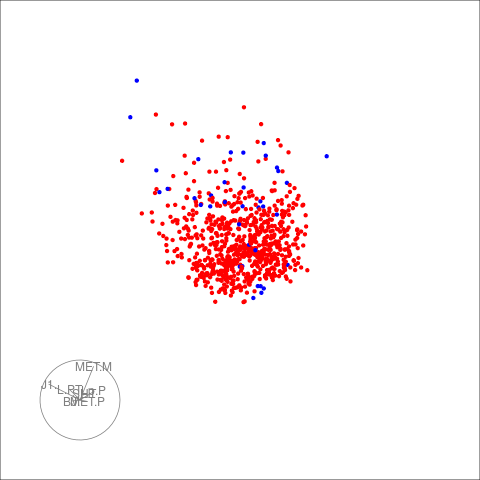
\includegraphics[width=\linewidth, keepaspectratio=true]{bm_I_false-001.png}
  \end{minipage}
  \begin{minipage}[htbp]{0.4\textwidth}
    \centering
    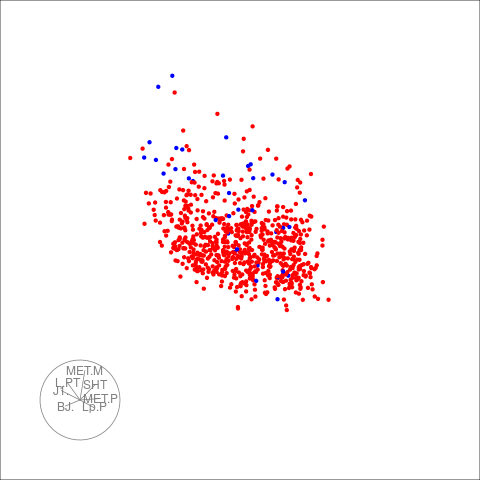
\includegraphics[width=\linewidth, keepaspectratio=true]{bm_I_false-012.png}
  \end{minipage}
  \begin{minipage}[htbp]{0.4\textwidth}
    \centering
    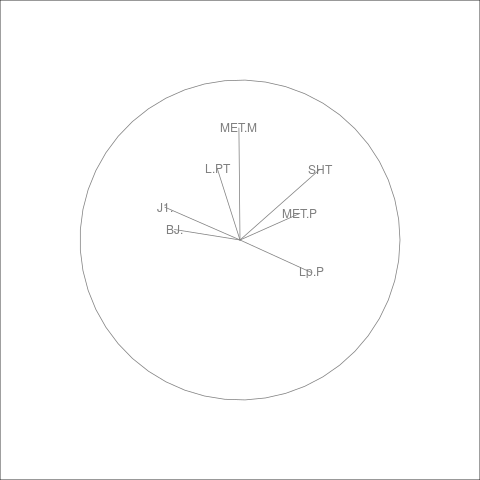
\includegraphics[width=\linewidth, keepaspectratio=true]{bm_I_false_axis.png}
  \end{minipage}
  \begin{minipage}[htbp]{0.4\textwidth}
    \centering
    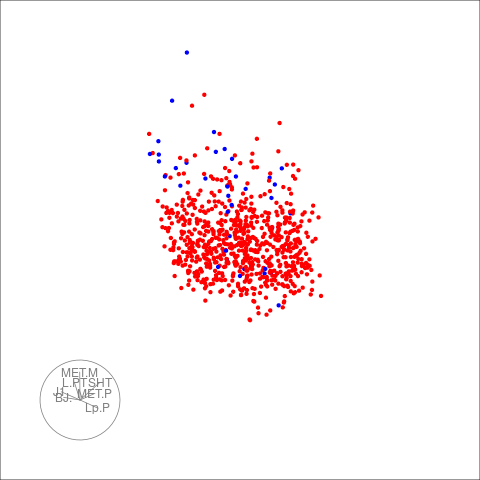
\includegraphics[width=\linewidth, keepaspectratio=true]{bm_I_false-024.png}
  \end{minipage}
  \caption{Guided tour of misclassified points in Benchmark 4: $m_{\Tilde{t}} = 750$ GeV and $m_{\Tilde{\chi}_1^0} = 1$ GeV. The signal events are in red and background events are in blue. The spread of both signal-like and background-like events make it difficult for the classifier to distinguish them.}
  \label{fig:bmInF_tour}
\end{figure}

\begin{figure}[htbp]
\centering
  \begin{minipage}[htbp]{0.4\textwidth}
    \centering
    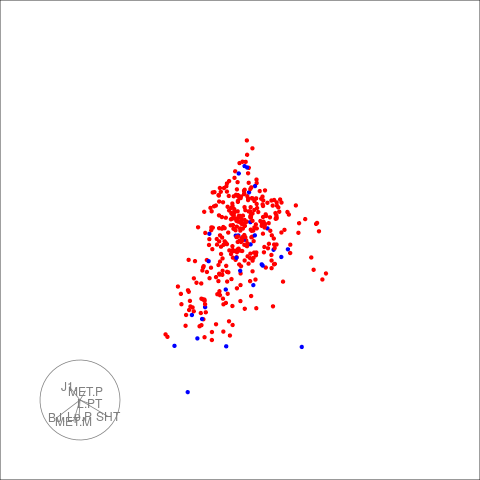
\includegraphics[width=\linewidth, keepaspectratio=true]{bm3_false-001.png}
  \end{minipage}
  \begin{minipage}[htbp]{0.4\textwidth}
    \centering
    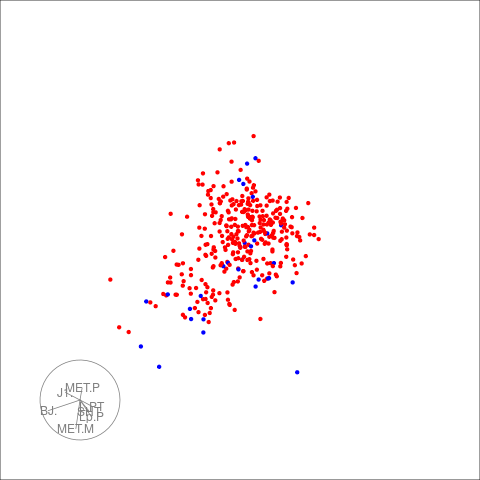
\includegraphics[width=\linewidth, keepaspectratio=true]{bm3_false-012.png}
  \end{minipage}
  \begin{minipage}[htbp]{0.4\textwidth}
    \centering
    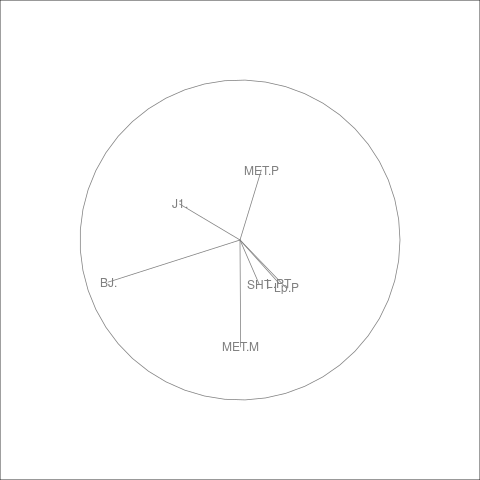
\includegraphics[width=\linewidth, keepaspectratio=true]{bm3_false_axis.png}
  \end{minipage}
  \begin{minipage}[htbp]{0.4\textwidth}
    \centering
    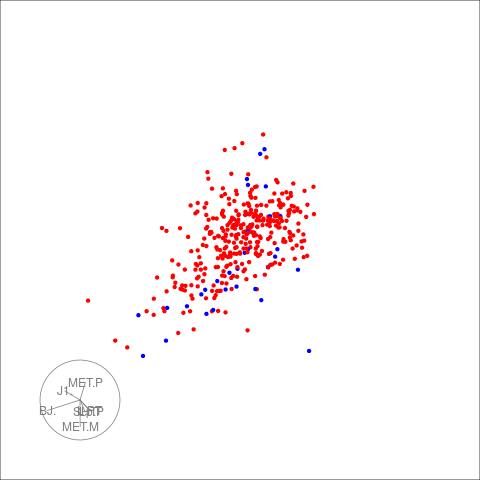
\includegraphics[width=\linewidth, keepaspectratio=true]{bm3_false-023.png}
  \end{minipage}
  \caption{Guided tour of misclassified points in Benchmark 3: $m_{\Tilde{t}} = 1.25$ TeV and $m_{\Tilde{\chi}_1^0} = 100$ GeV. The signal events are in red and background events are in blue. There is a similar distribution in the signal and background events, and due to the large sampling difference between the two signatures (as shown in Table \ref{tab:Values3}, it is difficult in this particular case to observe distinct patterns, unlike Figure \ref{fig:bmInF_tour}.}
  \label{fig:bm3F_tour}
\end{figure}
